\unnumberedChapter{Quad Block Controller}

The following section present our block controller. Each \textbf{block controller board} will have a main controller based board with the power module circuitry and RailCom detectors. This board alone will also cover all features needed for a booster node. In addition, the\textbf{ block controller extension board(s)} will cover the needs for occupancy detection, turnout and signal control. Depending on the hardware types, there are different turnouts and signal drivers. Again, we could design a separate extension board for the track occupancy and another one for the turnout and signal control. Both can be connected to the block controller main board.

For the design of the hardware module, there are two basic ways. As said, one way is to implement a central approach to the management of all the blocks, the other is a decentralized approach where each block is managed separately. Our block control system implements the latter. It is a decentralized system where a block controller manages two, perhaps four blocks. There is no real limit, but the more blocks are managed by one block controller, the more cabling is required, up to having one block controller managing all blocks, and thus we are back to a central approach. The requirements for a decentralized approach are that all components required to manage a block are bundled in the block controller and perhaps extension board.


While all this may sound like a hardware overkill, the occupancy detectors the turnout and signals drivers need to be in place anyhow. So are the boosters. There are only the number of power modules, one per block, instead of few boosters along the layout required. But having a power module for each bock gives us a good way to manage analog and digital blocks in one layout. And the prices for a H-Bridge chip that controls two blocks is quite reasonable so far.


\unnumberedSection{Block Diagram}

The following schematics show the block controller board for the quad block version. First, there is the main controller part with the connectors, the Raspberry PI PICO, the non-volatile memory, the CAN Bus line driver and the level shifters for the external connector pins used. Note that all the digital pins DIO0 to DIO7 are not exported, they are used on the board itself. The block controller also makes use of the track lane connector, which routes the track power signals from the block controller board to the extension board. This way, no extra cables need to be wired from block controller to extension board for this purpose. 

\begin{figure}[htbp]
    \centering
    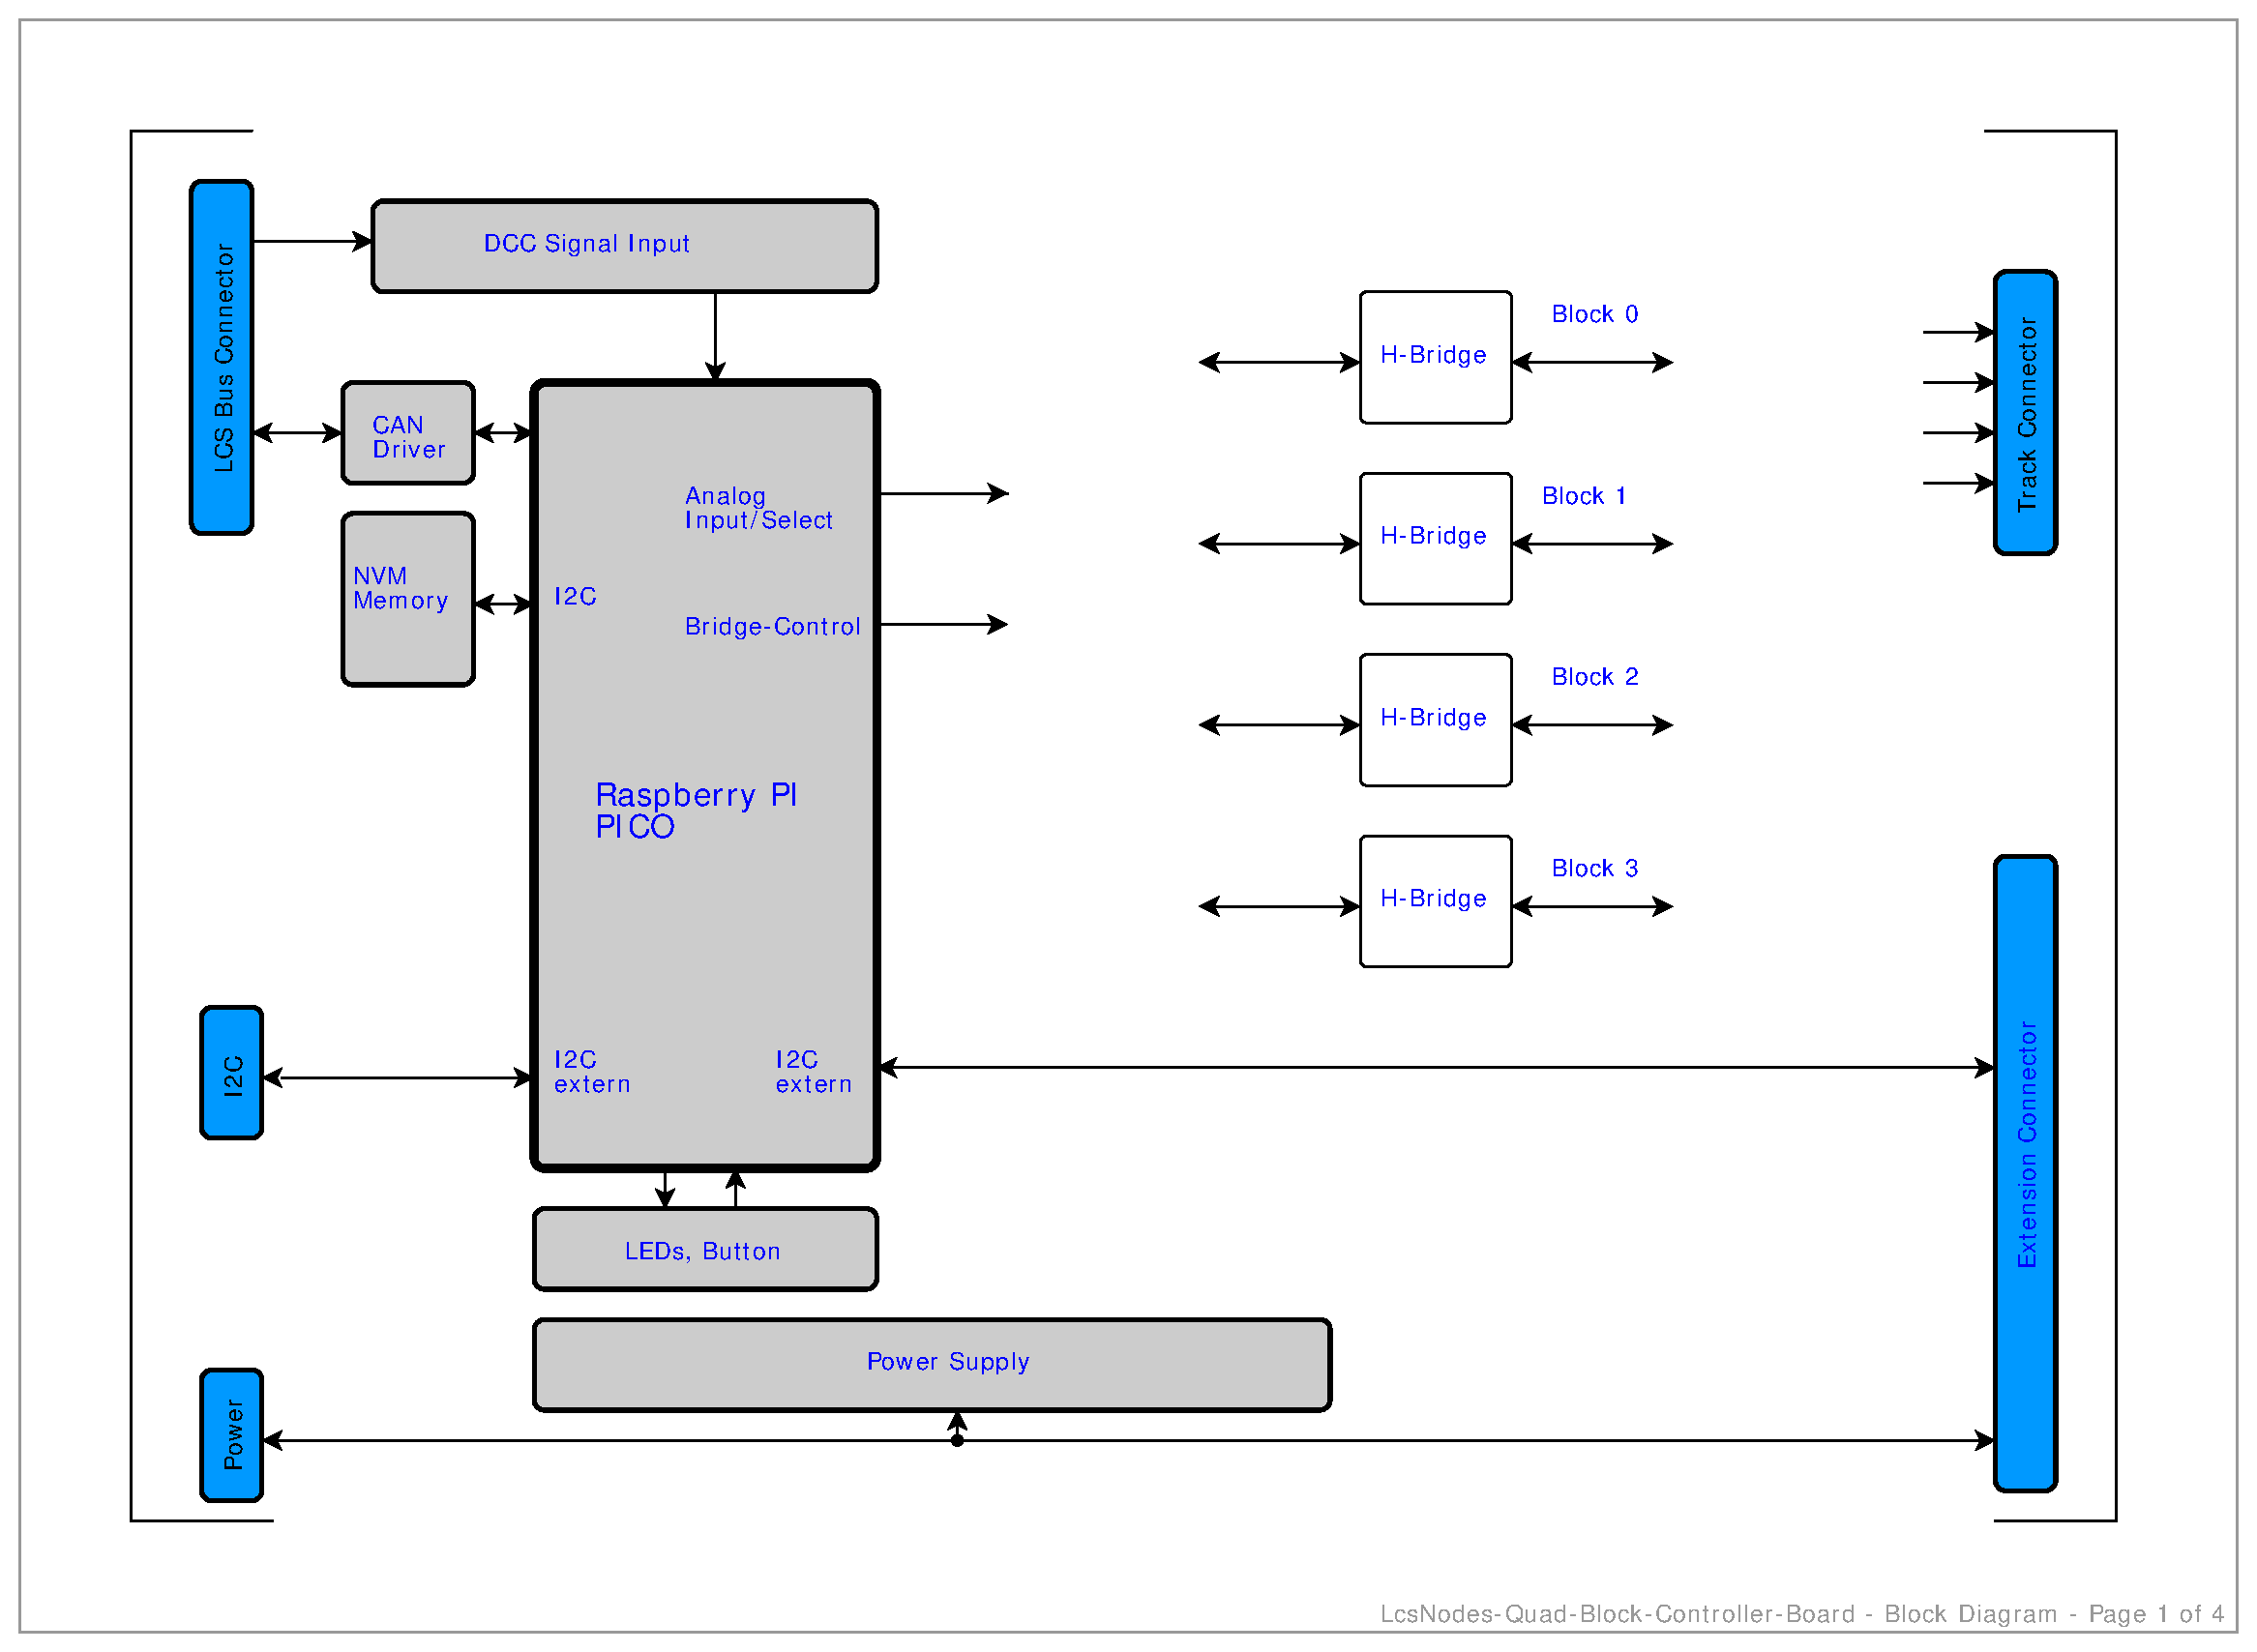
\includegraphics[page=1, width=0.9\textwidth]{./part-block-controller/chapter-quad-block-controller-hardware/Schematic_LcsNodes-Quad-Block-Controller-B.02.10.pdf}
    %\label{fig:schematic}
\end{figure}
\FloatBarrier

\unnumberedSection{Main Controller}

The first schematic shows the main controller Raspberry PI Pico, the level shifters required for the extension connector pins, the CAN bus driver and the non-volatile memory. This part is very similar to the main controller board shown in the previous chapters.

\begin{figure}[htbp]
    \centering
    \includegraphics[page=2, width=0.9\textwidth]{./part-block-controller/chapter-quad-block-controller-hardware/Schematic_LcsNodes-Quad-Block-Controller-B.02.10.pdf}
    \end{figure}
\FloatBarrier

The block controller will take the DCC signal and eventually feed it to the H-Bridge power module. On the input side, there is an opto-coupler. To cover the wide range of input voltages, there is a jumper to select the LED current limit resistor needed. For input ranges up to 10 volts a single resistor of 47O Ohm will do. Higher voltages as we seen the for HP to G-Scale add an 820 Ohm resistor.  


// ??? done in SW...

In addition to recognizing the DCC cutout situation, we need to worry about several block controllers receiving that signal slightly out of sync. Not all will switch into cutout mode at exactly the same time. When the boosters are slightly out of sync there could be. To address these issues, the signal detector will generate a short window of a few microseconds where the power module input signal is put in the "high impedance" state at the start of the cutout phase. Since the signal detector has no knowledge whether the booster is running in DCC or PWM mode, the short window will also take place in PWM mode, although not needed. Currently the implementation uses a window of about 4 microseconds.
 

\unnumberedSection{Power Unit}

Next is the power unit. The workings have already been described in the chapter on power units. The power unit is a H-Bridge with a current consumption measurement. The analog voltage across the shunt resistor is amplified and read in by the controller. Four H-Bridges need four analog inputs on the controller which we don't have on the Raspberry Pi PICO. All analog input signals are therefore multiplexed to one analog input port. We can thus read only one current measurement at a time.

\begin{figure}[htbp]
    \centering
    \includegraphics[page=3, width=0.9\textwidth]{./part-block-controller/chapter-quad-block-controller-hardware/Schematic_LcsNodes-Quad-Block-Controller-B.02.10.pdf}
    %\label{fig:schematic}
\end{figure}
\FloatBarrier

\unnumberedSection{Connector and Power Supply}

\begin{figure}[htbp]
    \centering
    \includegraphics[page=4, width=0.9\textwidth]{./part-block-controller/chapter-quad-block-controller-hardware/Schematic_LcsNodes-Quad-Block-Controller-B.02.10.pdf}
    %\label{fig:schematic}
\end{figure}
\FloatBarrier


\unnumberedSection{Quad Block Controller PCB}

The quad controller is implemented on a 10x16cm board layout. As you can see, it is a dense board. Even the place below the PICO board is used. Without SMD parts, this board would for sure not fit onto a 10x16Cm layout.

\begin{figure}[htbp]
    \centering
    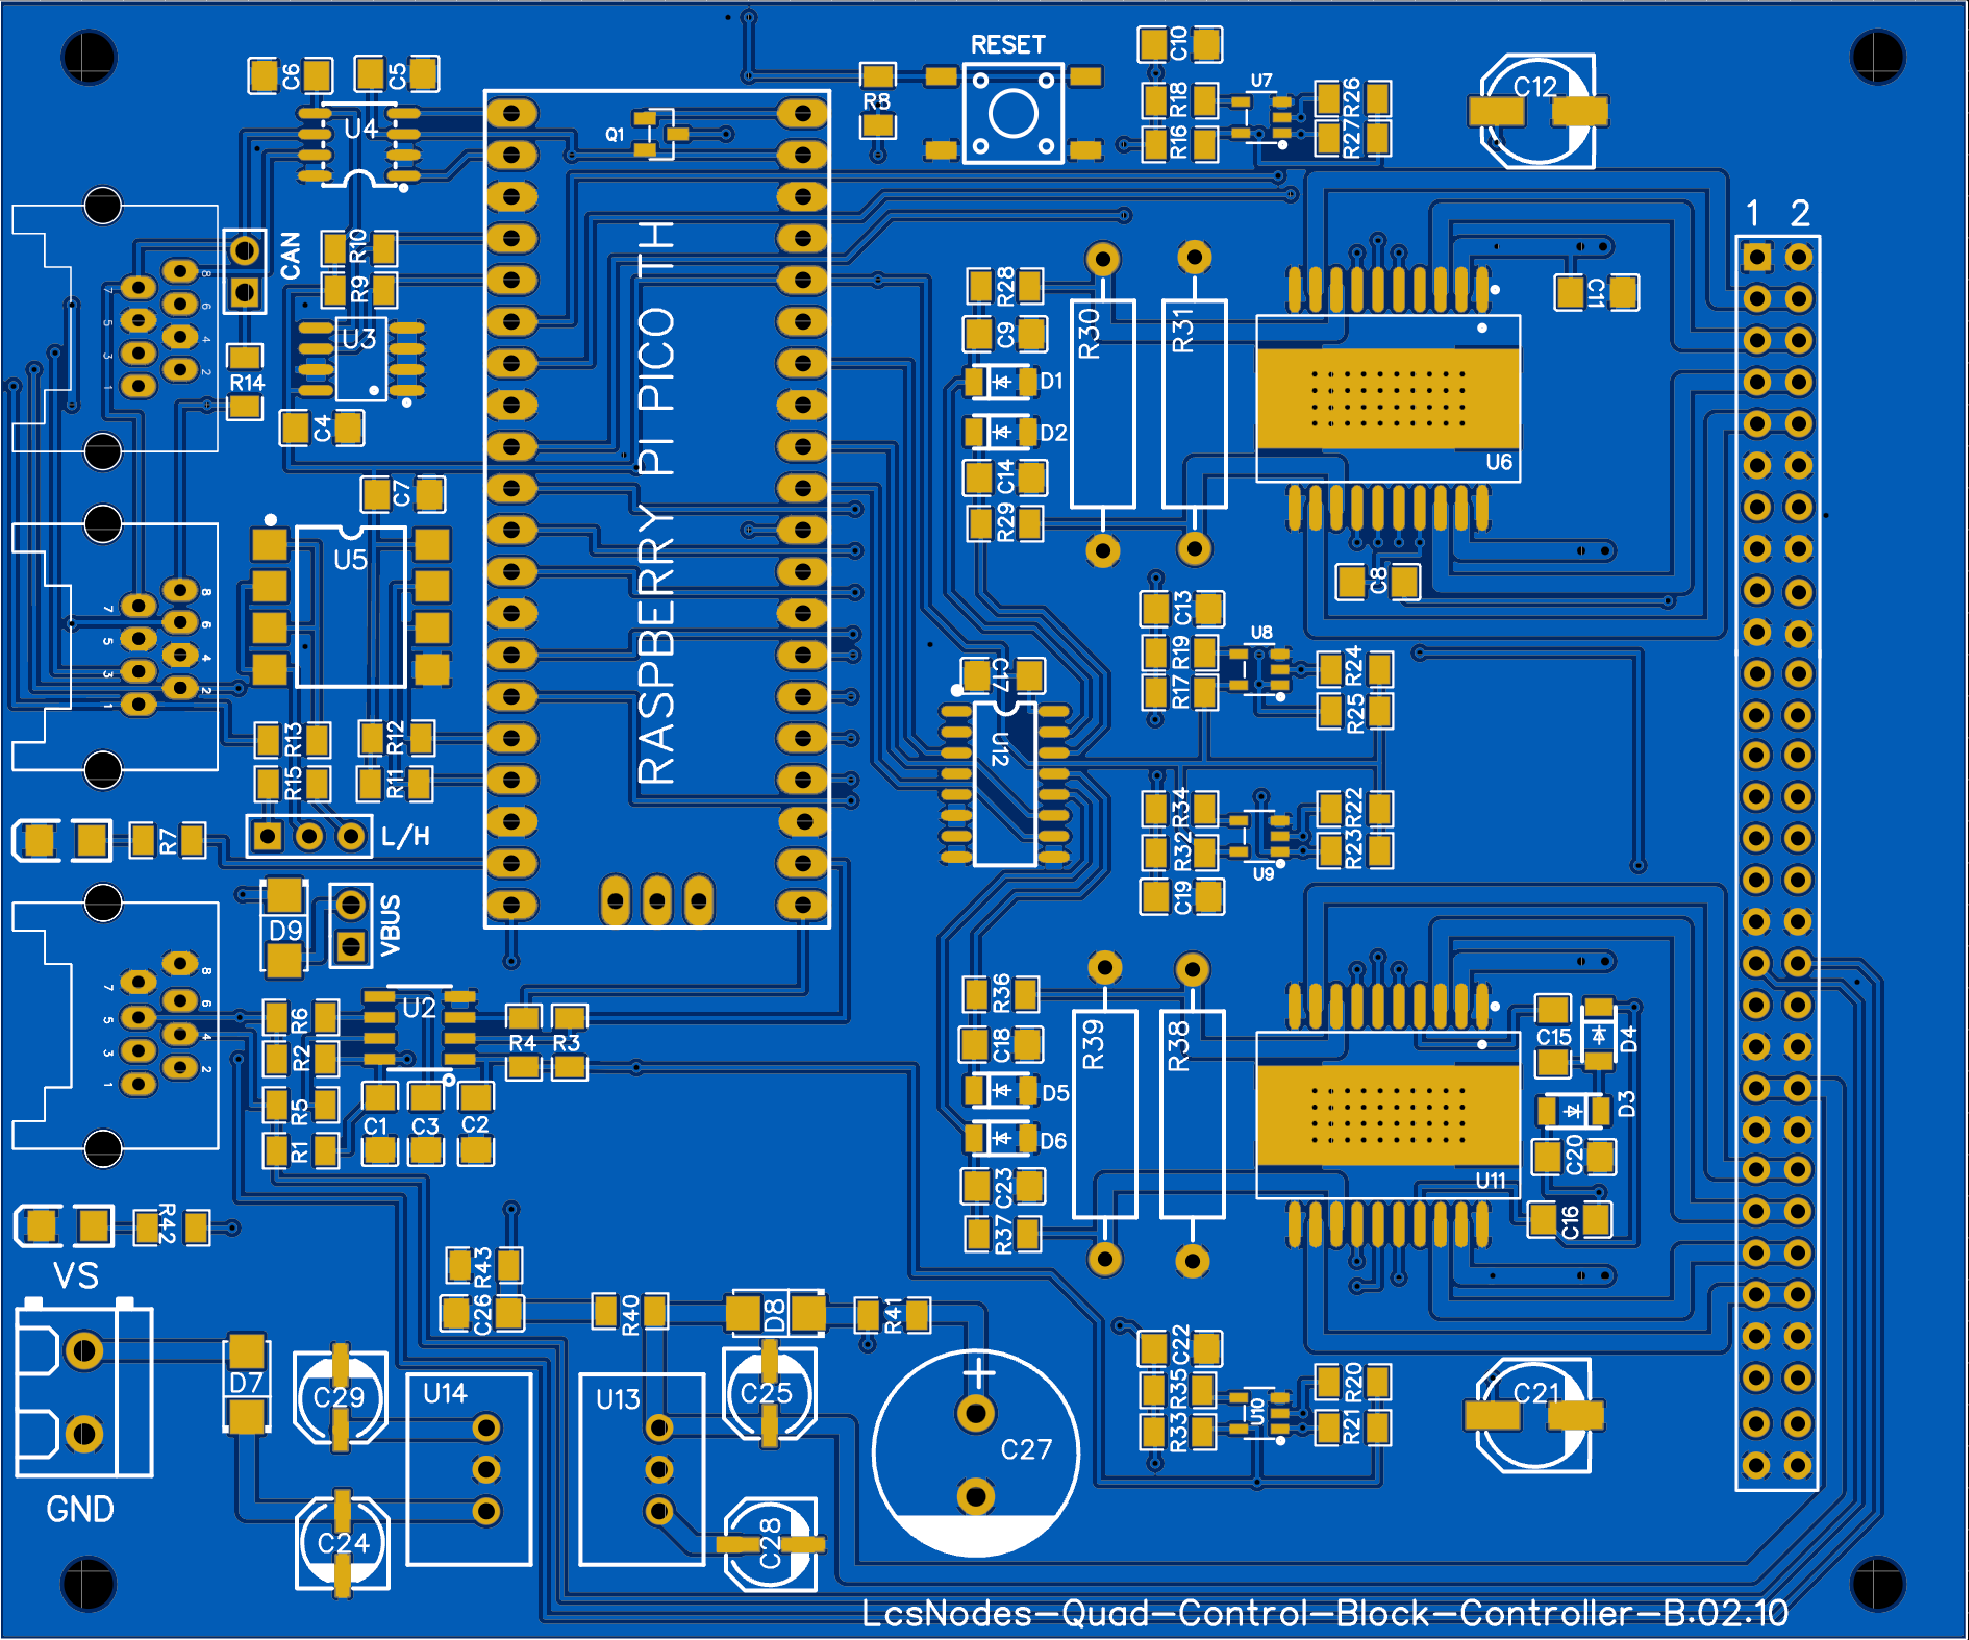
\includegraphics[width=0.9\textwidth]{./part-block-controller/chapter-quad-block-controller-hardware/PCB_LcsNodes-Quad-Block-Controller-B.02.10.pdf}
    \end{figure}
\FloatBarrier


Well, that is the quad block controller. It is so to speak a maximum configuration. When designing a block controller with just two blocks, just take out one H-Bridge mode decoder and one Railcom detector. Furthermore, the L6205 dual H-Bridge can be configured to deliver twice the amperage. For larger scales a version of the block controller needs to be available that delivers on two blocks 5.6 Amps. There could also be a board that just has one block, which would be a classical booster. There could also be a board that has a power H-Bridge piggybacked on top, and so on. This chapter showed a full fledged four channel version, other combinations would still rest on the same core building blocks described.


\unnumberedSection{H-Bridge control}

Both block controllers make use of a PICO feature. When looking at the Raspberry Pi PICO controller the PIO state machine is a highly versatile output controller. A specialized processor in itself. As already mentioned, the CAN bus interface is already implemented as a PIO program instead of the typical CAN bus controller peripheral. How about using the PIO state machines also for our H-Bridge control. 

The H-Bridge enable line is derived from the two  input control lines, using the unassigned state of "11" as putting the H-Bridge into disconnected mode. All it needs is a simple NAND gate. Control input "00" still puts the bridge into short circuit mode for the DCC cutout feature, "01" and "10" are still the PWM mode options. 

The DCC signals are routed to two input pins on the PICO. The PIO program uses them as input to detect the cutout period and also to pass on the DCC signal. Since a PIO program is a program, we can also just implement the quiet period at the beginning of the cutout period. In other words, the entire logic of DCC signal input and H-Bridge control moves into the PICO. This will reduce the component count of a block controller significantly.

The following code snippet show how that PIO program could be implemented.

\pagebreak[3] % Suggests to break page here if needed
\lstset{style=codesnippetstyle}
\begin{lstlisting}
;----------------------------------------------------------------
; DCC Signal Handler. The block controller uses a small PIO 
; program to control the H-Bridge when DCC mode is enabled. The 
, basic work of the PIO state machine is to relay the inverted 
; DCC input from the OptoCouplers to the output pins
; which drive the select input of the H-Bridge chip. 
; 
; When the DCC input signal drops to 0b00, we either have no 
; signal or the start of the Cutout period. We insert a four 
; microsecond delay, which gives some leeway when two boosters
; are not entirely in sync, although driven from the same DCC 
; signal. After this blackout DCC input is relayed to the output.
; In addition, the start and end of the cutout period is signaled 
; with the PIO state machine interrupt flags.
;
;----------------------------------------------------------------
.program h_bridge_signal_control

main_loop:
    mov x, pins            ; Copy input pins to X register
    mov pins, x            ; Mirror input to output

    ; Check for falling edge to 0b00 (start cutout)
    jmp !x, blackout_start ; Jump if both pins are 0
    jmp main_loop          ; Keep mirroring otherwise

blackout_start:
    set pins, 0b11         ; Emit 0b11 (Hi-Z) for blackout
    set y, 31              ; Load loop counter for delay (31 * 5 cycles per loop)

blackout_wait:
    jmp y--, blackout_wait ; 31 iterations * ~5 cycles = ~4 µs delay at 125 MHz
    irq set 4              ; Set IRQ flag on cutout start

    ; Wait for rising edge (end of cutout)

wait_rising:
    mov x, pins            ; Read pins again
    jmp !x, wait_rising    ; Loop while still 0b00

    irq set 5              ; Set IRQ flag on cutout end
    jmp main_loop          ; Return to main loop
    
\end{lstlisting}

\FloatBarrier


// ??? How do we do PWM ? it is done directly by the PICO... the PIO state machine pauses...
// ??? but we still need to sync on the cutout signal ...


\unnumberedSection{Summary}

This chapter presented the quad block controllers. 

// ??? uses PIO


From a firmware perspective, the bridge is controlled with two bits, putting the bridge in disconnected mode, PWM modes forward and reverse and finally DCC mode.

